\documentclass [a4paper] {article}

%% \usepackage[right=3cm, left=3cm]{geometry}

\usepackage[spanish]{babel} 
\usepackage[utf8]{inputenc} 
\usepackage{multirow} 
\usepackage{float} 

\title{R-PL2}
\author{Gabriel López, Sergio Sanz, Álvaro Zamorano}

\usepackage{Sweave}
\begin{document}

\maketitle

\graphicspath{ {./tmp/} }

\section{Ejercicio realizado en clase.}
Para poder usar el algoritmo \textbf{Apriori} y sus reglas de asociación vamos a utilizar el paquete
\texttt{arules}. Este paquete hay que descargarlo desde la página de CRAN y para instalarlo hay que
ejecutar el siguiente código:

\begin{Schunk}
\begin{Sinput}
> install.packages("./arules_1.6-4.zip",repos=NULL)
\end{Sinput}
\end{Schunk}

\bigskip
De esta forma, el paquete únicamente está instalado. Para poder usarlo es necesario cargarlo:
\begin{Schunk}
\begin{Sinput}
> library(arules)
\end{Sinput}
\end{Schunk}

Los datos a usar en este primer ejercicio se componen de 6 cestas de la compra, en concreto
estas son: \{Pan, Agua, Leche, Naranjas\},\{{Pan, Agua, Café, Leche\}, \{Pan, Agua, Leche\}, 
\{Pan, Café, Leche\}, \{Pan, Agua\}, \{Leche\}.

\bigskip
Para introducir estos datos en el algoritmo a usar es necesario crear una matriz con el siguiente
aspecto.
\begin{table}[H]
\begin{center}
\begin{tabular}{|c|c|c|c|c|c|}
\hline
Suceso & Pan & Agua & Café & Leche & Naranjas \\
\hline \hline
s1 & 1 & 1 & 0 & 1 & 1 \\ \hline
s2 & 1 & 1 & 1 & 1 & 0 \\ \hline
s3 & 1 & 1 & 0 & 1 & 0 \\ \hline
s4 & 1 & 0 & 1 & 1 & 0 \\ \hline
s5 & 1 & 1 & 0 & 0 & 0 \\ \hline
s6 & 0 & 0 & 0 & 1 & 0 \\ \hline
\end{tabular}
\end{center}
\end{table}

\bigskip
Esta matriz se introduce en R mediante:
\begin{Schunk}
\begin{Sinput}
> muestra<-Matrix(c(1,1,0,1,1,1,1,1,1,0,1,1,0,1,0,1,0,1,1,0,1,1,0,0,0,0,0,0,1,0),
+ 6,5,byrow=T,dimnames=list(c("suceso1","suceso2","suceso3","suceso4","suceso5",
+ "suceso6"),c("Pan","Agua","Cafe","Leche","Naranjas")),sparse=T)
\end{Sinput}
\end{Schunk}

\bigskip
Se necesita convertir la matriz a una matriz dispersa a través de la función \textbf{as} la cuál convierte un objeto a una determinada
clase, en este caso la clase es \textit{nsparseMatrix}. Esta clase lo que hace es cambiar los valores mayores de 0 por un valor binario, 
con el fin de gastar la menor cantidad de memoria posible ya que solo se almacenan aquellas posiciones no vacias, es decir, las que cuyo
valor es distinto de 0.
\begin{Schunk}
\begin{Sinput}
> muestrangCMatrix<-as(muestra,"nsparseMatrix")
\end{Sinput}
\end{Schunk}

\bigskip
El siguiente paso a realizar es calcular la \textbf{traspuesta} de la última matriz generada.
\begin{Schunk}
\begin{Sinput}
> transpuestangCMatrix<-t(muestrangCMatrix)
\end{Sinput}
\end{Schunk}

\bigskip
Antes de aplicar el algoritmo, calculamos y mostramos todas las \textbf{transacciones}, es decir, todas las asociaciones
que hay en nuestros datos.
\begin{Schunk}
\begin{Sinput}
> transacciones<-as(transpuestangCMatrix,"transactions")
> summary(transacciones)
\end{Sinput}
\begin{Soutput}
transactions as itemMatrix in sparse format with
 6 rows (elements/itemsets/transactions) and
 5 columns (items) and a density of 0.5666667 

most frequent items:
     Pan    Leche     Agua     Cafe Naranjas  (Other) 
       5        5        4        2        1        0 

element (itemset/transaction) length distribution:
sizes
1 2 3 4 
1 1 2 2 

   Min. 1st Qu.  Median    Mean 3rd Qu.    Max. 
  1.000   2.250   3.000   2.833   3.750   4.000 

includes extended item information - examples:
  labels
1    Pan
2   Agua
3   Cafe

includes extended transaction information - examples:
  itemsetID
1   suceso1
2   suceso2
3   suceso3
\end{Soutput}
\end{Schunk}

\bigskip
Por último, aplicamos el algoritmo \textbf{Apriori} para las asociaciones cuyo soporte sea igual o superior al 50\% y cuya confianza
sea igual o mayor que el 80\%.
\begin{Schunk}
\begin{Sinput}
> asociaciones<-apriori(transacciones,parameter=list(support=0.5,confidence=0.8))
\end{Sinput}
\end{Schunk}
\begin{Schunk}
\begin{Sinput}
> inspect(asociaciones)
\end{Sinput}
\begin{Soutput}
    lhs             rhs     support   confidence lift count
[1] {}           => {Leche} 0.8333333 0.8333333  1.00 5    
[2] {}           => {Pan}   0.8333333 0.8333333  1.00 5    
[3] {Agua}       => {Pan}   0.6666667 1.0000000  1.20 4    
[4] {Pan}        => {Agua}  0.6666667 0.8000000  1.20 4    
[5] {Leche}      => {Pan}   0.6666667 0.8000000  0.96 4    
[6] {Pan}        => {Leche} 0.6666667 0.8000000  0.96 4    
[7] {Agua,Leche} => {Pan}   0.5000000 1.0000000  1.20 3    
\end{Soutput}
\end{Schunk}

\bigskip
Se puede observar, a través de las transacciones las siguientes conclusiones:
\begin{enumerate}
\item Las personas que compran agua, compran también pan, y viceversa.
\item Las personas que compran leche, compran pan, y viceversa.
\item Las que compran agua y leche juntos también compran pan.
\end{enumerate}

%%%%%%%%%%%%%%%%%%%%%%%%%%%%%%%%%%%%%%%%%%%%%%%%%%%%%%%%%%%%%%%%%%%%%%%%%%%%%%%%%%%%%%%%%%%%%%%%%%%%%%%%%%%%%%%%%%%%%%%%%%%%%%%%%%%%%%%

\bigskip
\section{Parte 2.}
\subsection{Datos de ventas de coches.}
Para el leer el fichero \texttt{.txt} hemos creado una función la cuál nos devuelve una lista con las filas
de la matriz.
\begin{Schunk}
\begin{Sinput}
> source("leerMatriz.R")
> leerM
\end{Sinput}
\begin{Soutput}
function(ruta) {

    data<-read.table(ruta,header=TRUE)
    mat<-as.matrix(data)
    sz<-dim(mat)
    l<-c()

    for (i in 1:sz[1]) {
        for (j in 1:sz[2]){
            l<-c(l,mat[i,j])
        }
    }

    return(l)
}
\end{Soutput}
\end{Schunk}

Procedemos a la lectura de dicho fichero.
\begin{Schunk}
\begin{Sinput}
> m<-leerM("2_1.txt")
\end{Sinput}
\end{Schunk}

\bigskip
La matriz leida tiene el siguiente aspecto.
\begin{table}[H]
\begin{center}
\begin{tabular}{|c|c|c|c|c|c|c|}
\hline
Suceso & Xenon & Alarma & Techo & Navegador & Bluetooth & ControlV \\
\hline \hline
s1 & 1 & 0 & 0 & 1 & 1 & 1 \\ \hline
s2 & 1 & 0 & 1 & 0 & 1 & 1 \\ \hline
s3 & 1 & 0 & 0 & 1 & 0 & 1 \\ \hline
s4 & 1 & 0 & 1 & 1 & 1 & 0 \\ \hline
s5 & 1 & 0 & 0 & 0 & 1 & 1 \\ \hline
s6 & 0 & 0 & 0 & 1 & 0 & 0 \\ \hline
s7 & 1 & 0 & 0 & 0 & 1 & 1 \\ \hline
s8 & 0 & 1 & 1 & 0 & 0 & 0 \\ \hline
\end{tabular}
\end{center}
\end{table}

\bigskip
Esta matriz se introduce en R mediante:
\begin{Schunk}
\begin{Sinput}
> mCoches<-Matrix(m,8,6,byrow=T,dimnames=list(c("suceso1","suceso2","suceso3",
+ "suceso4","suceso5","suceso6", "suceso7", "suceso8"),
+ c("Xenon", "Alarma", "Techo", "Navegador", "Bluetooth", "ControlV")),sparse=T)
\end{Sinput}
\end{Schunk}

\bigskip
Se necesita convertir la matriz a una matriz dispersa a través de la función \textbf{as}.
\begin{Schunk}
\begin{Sinput}
> mCochesngC<-as(mCoches,"nsparseMatrix")
\end{Sinput}
\end{Schunk}

\bigskip
El siguiente paso a realizar es calcular la \textbf{traspuesta} de la última matriz generada.
\begin{Schunk}
\begin{Sinput}
> transpuestangC<-t(mCochesngC)
\end{Sinput}
\end{Schunk}

\bigskip
Antes de aplicar el algoritmo, calculamos y mostramos todas las \textbf{transacciones}, es decir, todas las asociaciones
que hay en nuestros datos.
\begin{Schunk}
\begin{Sinput}
> transac<-as(transpuestangC,"transactions")
> summary(transac)
\end{Sinput}
\begin{Soutput}
transactions as itemMatrix in sparse format with
 8 rows (elements/itemsets/transactions) and
 6 columns (items) and a density of 0.5 

most frequent items:
    Xenon Bluetooth  ControlV Navegador     Techo   (Other) 
        6         5         5         4         3         1 

element (itemset/transaction) length distribution:
sizes
1 2 3 4 
1 1 3 3 

   Min. 1st Qu.  Median    Mean 3rd Qu.    Max. 
   1.00    2.75    3.00    3.00    4.00    4.00 

includes extended item information - examples:
  labels
1  Xenon
2 Alarma
3  Techo

includes extended transaction information - examples:
  itemsetID
1   suceso1
2   suceso2
3   suceso3
\end{Soutput}
\end{Schunk}

\bigskip
Por último, aplicamos el algoritmo \textbf{Apriori} para las asociaciones cuyo soporte sea igual o superior al 40\% y cuya confianza
sea igual o mayor que el 90\%.
\begin{Schunk}
\begin{Sinput}
> asoc<-apriori(transac,parameter=list(support=0.4,confidence=0.9))
\end{Sinput}
\end{Schunk}
\begin{Schunk}
\begin{Sinput}
> inspect(asoc)
\end{Sinput}
\begin{Soutput}
    lhs                     rhs     support confidence lift     count
[1] {ControlV}           => {Xenon} 0.625   1          1.333333 5    
[2] {Bluetooth}          => {Xenon} 0.625   1          1.333333 5    
[3] {Bluetooth,ControlV} => {Xenon} 0.500   1          1.333333 4    
\end{Soutput}
\end{Schunk}

\bigskip
Igual que en el caso anterior, a través de las transacciones obtenidas se pueden obtener las siguientes conclusiones: los 
coches que incorporan tanto control de velocidad y/o bluetooth, tienen luces de Xenon.

%%%%%%%%%%%%%%%%%%%%%%%%%%%%%%%%%%%%%%%%%%%%%%%%%%%%%%%%%%%%%%%%%%%%%%%%%%%%%%%%%%%%%%%%%%%%%%%%%%%%%%%%%%%%%%%%%%%%%%%%%%%%%%%%%%%%%%%

\bigskip
\subsection{Desarrollo del grupo.}
Para el desarrolo de esta parte hemos buscado unos datos en \textit{Kaggle} correspondientes a carros de la compra aleatorios.

En primer lugar procedemos a leer los datos que hay en el fichero \texttt{.csv} almacenándolos directamente
en un objeto de tipo \textbf{transactions} ya que es la estructura de almacenamiento empleada por \textit{arules.}
Para poder leer estos datos es necesario tener cargada la librería mediante \texttt{library(arules)}, como se ha
indicado anteriormente.

Las transacciones se leen gracias al uso de la función \textbf{read.transactions}.
\begin{Schunk}
\begin{Sinput}
> shopT<-read.transactions("shop.csv", format = "basket", 
+                   header = FALSE, sep = ",", 
+                   cols = NULL, rm.duplicates = FALSE, 
+                   skip = 0)
\end{Sinput}
\end{Schunk}

\bigskip
Una vez leídas las transacciones, mostramos un ejemplo de ellas:
\begin{Schunk}
\begin{Sinput}
> inspect(shopT[1])
\end{Sinput}
\begin{Soutput}
    items              
[1] {all- purpose,     
     aluminum foil,    
     beef,             
     butter,           
     dinner rolls,     
     flour,            
     ice cream,        
     laundry detergent,
     lunch meat,       
     mixes,            
     pork,             
     sandwich bags,    
     shampoo,          
     soap,             
     soda,             
     vegetables,       
     yogurt}           
\end{Soutput}
\end{Schunk}

\bigskip
Observamos en un gráfico el \textbf{soporte} de los 10 productos más comprados, es decir, en cuantos
sucesos aparece cada uno de los productos respecto al total de sucesos.
\begin{Schunk}
\begin{Sinput}
> source("sopImg.R")
> d<-sopImg(shopT,10,"sopI.png")
\end{Sinput}
\end{Schunk}
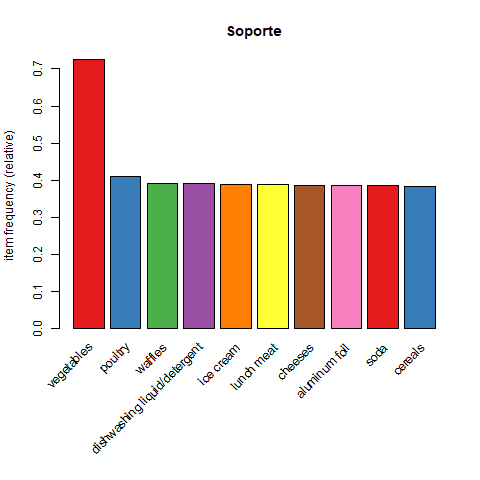
\includegraphics[width=\textwidth]{sopI}

Para usar la función anterior es necesario installar e importar mediante \texttt{library} un paquete de R
que nos ofrece el uso de la paleta de colores empleada en el gráfico. Dicha función tiene el siguiente
aspecto:
\begin{Schunk}
\begin{Sinput}
> sopImg
\end{Sinput}
\begin{Soutput}
function(data, n, ruta) {

    install.packages("RColorBrewer")
    library(RColorBrewer)

    png(paste("./tmp/",ruta,sep=""))

    itemFrequencyPlot(data, topN=n, col=brewer.pal(8,'Set1'),
        type="relative",main="Soporte")

    dev.off()
}
\end{Soutput}
\end{Schunk}

\bigskip
Estudiando la documentación perteneciente a la librería arules, hemos encontrado una función con la que extraer
conjuntos de elementos frecuentes de acuerdo a un soporte dado. Está función es \textbf{eclat.}
Respecto al algoritmo Apriori se puede decir que reduce el tiempo de cómputo a causa de sacrificar memoria; su
forma de actuar es almacenar para cada item en qué transacciones aparece (de forma vertical), por tanto, 
se diferencian en la manera de escanear y analizar los datos.

\bigskip
Procedemos a su ejecución:
\begin{Schunk}
\begin{Sinput}
> is<-eclat(shopT,parameter=list(support=0.3))
\end{Sinput}
\end{Schunk}

\bigskip
La función comentada anteriormente nos proporciona un objeto de la clase \texttt{itemsets}, y gracias a la función
\textbf{ruleInduction} podemos obtener las asociaciones que contienen nuestros datos. RuleInduction induce todas las reglas 
que puede generar el conjunto de conjuntos de elementos (itemsets) a partir de un conjunto transacciones.
\begin{Schunk}
\begin{Sinput}
> rules<-ruleInduction(is,shopT,confidence=0.7)
> inspect(rules)
\end{Sinput}
\begin{Soutput}
     lhs                               rhs          support  
[1]  {laundry detergent}            => {vegetables} 0.3042028
[2]  {yogurt}                       => {vegetables} 0.3082055
[3]  {eggs}                         => {vegetables} 0.3108739
[4]  {ice cream}                    => {vegetables} 0.3008672
[5]  {lunch meat}                   => {vegetables} 0.3015344
[6]  {waffles}                      => {vegetables} 0.3048699
[7]  {cheeses}                      => {vegetables} 0.3035357
[8]  {aluminum foil}                => {vegetables} 0.3095397
[9]  {dishwashing liquid/detergent} => {vegetables} 0.3048699
[10] {poultry}                      => {vegetables} 0.3202135
     confidence lift     itemset
[1]  0.8099467  1.114885  1     
[2]  0.8148148  1.121586  2     
[3]  0.8146853  1.121408  3     
[4]  0.7722603  1.063010  4     
[5]  0.7766323  1.069028  5     
[6]  0.7785349  1.071647  6     
[7]  0.7844828  1.079834  7     
[8]  0.8013817  1.103096  8     
[9]  0.7811966  1.075311  9     
[10] 0.7830343  1.077841 10     
\end{Soutput}
\end{Schunk}

\bigskip
Una vez obtenidas las asociaciones que contienen nuestros datos, vamos a mostrarlas de forma gráfica para que las conclusiones
se puedan obtener de una forma más sencilla y visual.

\bigskip
En primer lugar, para poder usar los gráficos instalaremos el paquete \textit{arulesViz}, como se ha explicado en numerosas
ocasiones.
\begin{Schunk}
\begin{Sinput}
> install.packages("arulesViz")
> library(arulesViz)
\end{Sinput}
\end{Schunk}

\bigskip
En el siguiente gráfico se muestran las asociaciones entre los productos de nuestra muestra de datos. El tamaño de los nodos
refleja el soporte de cada uno de los productos y el color de los mismos, la relación de elevación (lift). Dicho lift representa 
la relación entre la confianza y la confianza esperada, es decir, un lift mayor que 1.0 implica que la relación entre el antecedente 
y el consecuente es más significativa de lo que se esperaría si los dos conjuntos fueran independientes, por tanto, cuanto mayor
sea la relación de elevación, más significativa será la asociación estudiada.
\begin{Schunk}
\begin{Sinput}
> source("graph.R")
> graph(rules,"graphR.png")
\end{Sinput}
\end{Schunk}
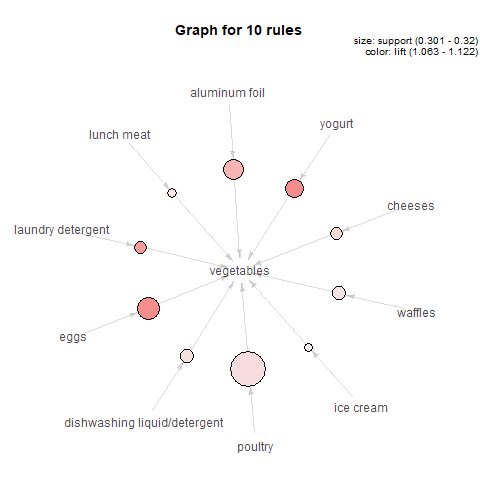
\includegraphics[width=\textwidth]{graphR}

\bigskip
La función usada para generar el gráfico anterior tiene la siguiente forma:
\begin{Schunk}
\begin{Sinput}
> graph
\end{Sinput}
\begin{Soutput}
function(rules, ruta) {

    png(paste("./tmp/",ruta,sep=""))

    plot(rules,method="graph",control=list(type="items"))

    dev.off()
}
\end{Soutput}
\end{Schunk}

\bigskip
Se puede observar lo siguiente: 
\begin{enumerate}
\item Pouldry es el producto con mayor soporte, seguido por eggs y aluminum foil.
\item Laundry detergent es el producto con mayor relación de elevación (lift), seguido por yogurt y eggs.
\item Todas los productos están asociados entorno a vegetables. Esto se debe en gran medida al soporte de vegetables
en el total de transacciones.
\end{enumerate}

\bigskip
A la vista de los resultados obtenidos con estos datos donde hay que usar un bajo soporte para obtener un cierto 
número de asociaciones, procedemos a hacer el análisis de un conjunto de datos contenido en arules. El dataset a usar es
\textit{Adult}

\bigskip
En primer lugar debemos cargar estos datos.
\begin{Schunk}
\begin{Sinput}
> data("Adult")
\end{Sinput}
\end{Schunk}

\bigskip
Estos datos tienen las siguientes columnas:
\begin{itemize}
\item Age
\item Workclass
\item Education
\item Education-num
\item Marital-status
\item Occupation
\item Relationship
\item Race
\item Sex
\item Capital-gain
\item Capital-loss
\item Fnlwgt
\item Hours-per-week
\item Native country
\item Income
\end{itemize}

\bigskip
Procedemos a realizar el análisis mediante el uso de eclat.
\begin{Schunk}
\begin{Sinput}
> isA<-eclat(Adult,parameter=list(support=0.5))
> rulesA<-ruleInduction(isA,Adult,confidence=0.9)
\end{Sinput}
\end{Schunk}

\scriptsize
\begin{Schunk}
\begin{Sinput}
> inspect(rulesA)
\end{Sinput}
\begin{Soutput}
     lhs                               rhs                              support confidence      lift itemset
[1]  {capital-loss=None,                                                                                    
      hours-per-week=Full-time}     => {capital-gain=None}            0.5191638  0.9259787 1.0093657       1
[2]  {capital-gain=None,                                                                                    
      hours-per-week=Full-time}     => {capital-loss=None}            0.5191638  0.9550659 1.0018756       1
[3]  {hours-per-week=Full-time}     => {capital-loss=None}            0.5606650  0.9582531 1.0052191       2
[4]  {hours-per-week=Full-time}     => {capital-gain=None}            0.5435895  0.9290688 1.0127342       3
[5]  {sex=Male,                                                                                             
      capital-loss=None,                                                                                    
      native-country=United-States} => {race=White}                   0.5113632  0.9032585 1.0563898       5
[6]  {race=White,                                                                                           
      sex=Male,                                                                                             
      native-country=United-States} => {capital-loss=None}            0.5113632  0.9442722 0.9905529       5
[7]  {race=White,                                                                                           
      sex=Male,                                                                                             
      capital-loss=None}            => {native-country=United-States} 0.5113632  0.9190124 1.0240556       5
[8]  {race=White,                                                                                           
      sex=Male}                     => {capital-loss=None}            0.5564268  0.9457804 0.9921350       6
[9]  {race=White,                                                                                           
      sex=Male}                     => {capital-gain=None}            0.5313050  0.9030799 0.9844048       7
[10] {sex=Male,                                                                                             
      native-country=United-States} => {race=White}                   0.5415421  0.9051090 1.0585540       8
[11] {race=White,                                                                                           
      sex=Male}                     => {native-country=United-States} 0.5415421  0.9204803 1.0256912       8
[12] {sex=Male,                                                                                             
      capital-gain=None,                                                                                    
      native-country=United-States} => {capital-loss=None}            0.5084149  0.9404636 0.9865576       9
[13] {sex=Male,                                                                                             
      native-country=United-States} => {capital-loss=None}            0.5661316  0.9462068 0.9925823      10
[14] {sex=Male,                                                                                             
      native-country=United-States} => {capital-gain=None}            0.5406003  0.9035349 0.9849008      11
[15] {sex=Male,                                                                                             
      capital-gain=None}            => {capital-loss=None}            0.5696941  0.9415288 0.9876750      12
[16] {sex=Male}                     => {capital-loss=None}            0.6331027  0.9470750 0.9934931      13
[17] {sex=Male}                     => {capital-gain=None}            0.6050735  0.9051455 0.9866565      14
[18] {workclass=Private,                                                                                    
      race=White,                                                                                           
      native-country=United-States} => {capital-loss=None}            0.5181401  0.9535418 1.0002768      17
[19] {workclass=Private,                                                                                    
      race=White,                                                                                           
      capital-loss=None}            => {native-country=United-States} 0.5181401  0.9130498 1.0174114      17
[20] {workclass=Private,                                                                                    
      race=White,                                                                                           
      capital-loss=None}            => {capital-gain=None}            0.5204742  0.9171628 0.9997559      18
[21] {workclass=Private,                                                                                    
      race=White,                                                                                           
      capital-gain=None}            => {capital-loss=None}            0.5204742  0.9511000 0.9977153      18
[22] {workclass=Private,                                                                                    
      race=White}                   => {capital-loss=None}            0.5674829  0.9549683 1.0017732      19
[23] {workclass=Private,                                                                                    
      race=White}                   => {capital-gain=None}            0.5472339  0.9208931 1.0038221      20
[24] {workclass=Private,                                                                                    
      race=White}                   => {native-country=United-States} 0.5433848  0.9144157 1.0189334      21
[25] {workclass=Private,                                                                                    
      capital-loss=None,                                                                                    
      native-country=United-States} => {capital-gain=None}            0.5414807  0.9182030 1.0008898      22
[26] {workclass=Private,                                                                                    
      capital-gain=None,                                                                                    
      native-country=United-States} => {capital-loss=None}            0.5414807  0.9517075 0.9983526      22
[27] {workclass=Private,                                                                                    
      native-country=United-States} => {capital-loss=None}            0.5897179  0.9554818 1.0023119      23
[28] {workclass=Private,                                                                                    
      native-country=United-States} => {capital-gain=None}            0.5689570  0.9218444 1.0048592      24
[29] {workclass=Private,                                                                                    
      capital-loss=None}            => {capital-gain=None}            0.6111748  0.9204465 1.0033354      25
[30] {workclass=Private,                                                                                    
      capital-gain=None}            => {capital-loss=None}            0.6111748  0.9529145 0.9996188      25
[31] {workclass=Private}            => {capital-loss=None}            0.6639982  0.9564974 1.0033773      26
[32] {workclass=Private}            => {capital-gain=None}            0.6413742  0.9239073 1.0071078      27
[33] {race=White,                                                                                           
      capital-loss=None,                                                                                    
      native-country=United-States} => {capital-gain=None}            0.6803980  0.9083504 0.9901500      30
[34] {race=White,                                                                                           
      capital-gain=None,                                                                                    
      native-country=United-States} => {capital-loss=None}            0.6803980  0.9457029 0.9920537      30
[35] {race=White,                                                                                           
      capital-gain=None,                                                                                    
      capital-loss=None}            => {native-country=United-States} 0.6803980  0.9189249 1.0239581      30
[36] {race=White,                                                                                           
      native-country=United-States} => {capital-loss=None}            0.7490480  0.9504325 0.9970152      31
[37] {race=White,                                                                                           
      capital-loss=None}            => {native-country=United-States} 0.7490480  0.9205626 1.0257830      31
[38] {race=White,                                                                                           
      native-country=United-States} => {capital-gain=None}            0.7194628  0.9128933 0.9951019      32
[39] {race=White,                                                                                           
      capital-gain=None}            => {native-country=United-States} 0.7194628  0.9202807 1.0254689      32
[40] {race=White,                                                                                           
      capital-loss=None}            => {capital-gain=None}            0.7404283  0.9099693 0.9919147      33
[41] {race=White,                                                                                           
      capital-gain=None}            => {capital-loss=None}            0.7404283  0.9470983 0.9935175      33
[42] {race=White}                   => {capital-loss=None}            0.8136849  0.9516307 0.9982720      34
[43] {race=White}                   => {capital-gain=None}            0.7817862  0.9143240 0.9966616      35
[44] {race=White}                   => {native-country=United-States} 0.7881127  0.9217231 1.0270761      36
[45] {capital-loss=None,                                                                                    
      native-country=United-States} => {capital-gain=None}            0.7793702  0.9117168 0.9938195      37
[46] {capital-gain=None,                                                                                    
      native-country=United-States} => {capital-loss=None}            0.7793702  0.9481891 0.9946618      37
[47] {native-country=United-States} => {capital-loss=None}            0.8548380  0.9525461 0.9992323      38
[48] {native-country=United-States} => {capital-gain=None}            0.8219565  0.9159062 0.9983862      39
[49] {capital-loss=None}            => {capital-gain=None}            0.8706646  0.9133376 0.9955863      40
[50] {capital-gain=None}            => {capital-loss=None}            0.8706646  0.9490705 0.9955863      40
\end{Soutput}
\end{Schunk}

\normalsize
\bigskip
Al igual que anteriormente, mostramos de forma gráfica las asociaciones obtenidas.
\begin{Schunk}
\begin{Sinput}
> graph(rulesA,"graphRA.png")
\end{Sinput}
\end{Schunk}
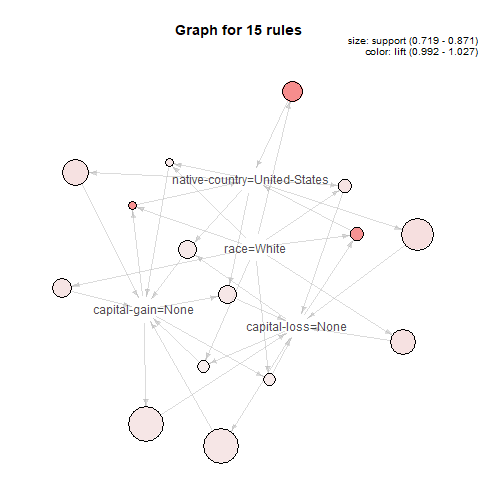
\includegraphics[width=\textwidth]{graphRA}

\bigskip
Para no tener en cuenta en las asociaciones los sucesos con capital-gain y capital-loss a None, 
mediante el uso de la función Apriori hemos eliminado dichos sucesos haciendo un filtro a través
del parámetro \texttt{appearance.}
\begin{Schunk}
\begin{Sinput}
> apr<-apriori(Adult,parameter=list(support=0.5,confidence=0.9),
+     appearance=list(none=c("capital-gain=None","capital-loss=None")))
\end{Sinput}
\end{Schunk}

\bigskip
Procedemos a mostrar las asociaciones obtenidas, tanto según lo representa la función \textit{inspect}, como 
de manera gráfica, haciendo uso de la función definida anteriormente.
\footnotesize
\begin{Schunk}
\begin{Sinput}
> inspect(apr)
\end{Sinput}
\begin{Soutput}
    lhs                               rhs                              support confidence     lift count
[1] {race=White}                   => {native-country=United-States} 0.7881127  0.9217231 1.027076 38493
[2] {race=White,                                                                                        
     sex=Male}                     => {native-country=United-States} 0.5415421  0.9204803 1.025691 26450
[3] {sex=Male,                                                                                          
     native-country=United-States} => {race=White}                   0.5415421  0.9051090 1.058554 26450
[4] {workclass=Private,                                                                                 
     race=White}                   => {native-country=United-States} 0.5433848  0.9144157 1.018933 26540
\end{Soutput}
\end{Schunk}

\normalsize
\begin{Schunk}
\begin{Sinput}
> graph(apr,"graphRP.png")
\end{Sinput}
\end{Schunk}
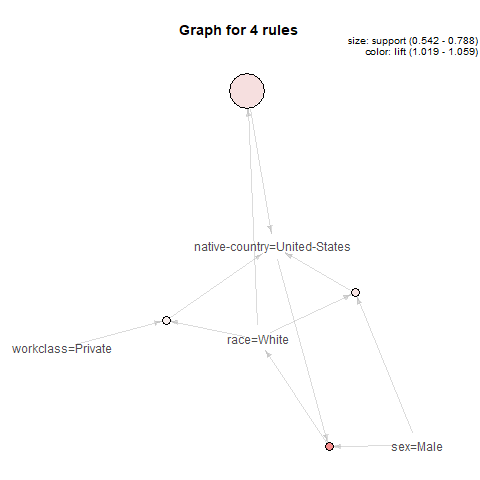
\includegraphics[width=\textwidth]{graphRP}

\bigskip
A partir de lo obtenido se puede concluir que:
\begin{enumerate}
\item Todas las personas de raza blanca y/o sexo masculino son de EEUU, y viceversa.
\item Las personas que trabajan en el sector privado y son de raza blanca, son de EEUU.
\end{enumerate}

\end{document}
